\documentclass{beamer}

\mode<presentation>
{
  \usetheme{CambridgeUS}
  \setbeamercovered{transparent}
}

\usepackage[english]{babel}
\usepackage[latin1]{inputenc}
\usepackage{times}
\usepackage[T1]{fontenc} 
% Or whatever. Note that the encoding and the font should match. If T1
% does not look nice, try deleting the line with the fontenc.
\usepackage{amsmath}

\newcommand{\linespace}{\vskip 0.25cm}

\definecolor{MyForestGreen}{rgb}{0,0.7,0} 
\newcommand{\tableemph}[1]{{#1}}
\newcommand{\tablewin}[1]{\tableemph{#1}}
\newcommand{\tablemid}[1]{\tableemph{#1}}
\newcommand{\tablelose}[1]{\tableemph{#1}}

\definecolor{MyLightGray}{rgb}{0.6,0.6,0.6}
\newcommand{\tabletie}[1]{\color{MyLightGray} {#1}}

% The text in square brackets is the short version of your title and will be used in the
% header/footer depending on your theme.
\title[CNNs in Medical Imaging]{Convolutional Neural Networks \\ in Medical Imaging}

% Sub-titles are optional - uncomment and edit the next line if you want one.
% \subtitle{Why does sub-tree crossover work?} 

% The text in square brackets is the short version of your name(s) and will be used in the
% header/footer depending on your theme.
\author[Finzel]{Mitchell Finzel}

% The text in square brackets is the short version of your institution and will be used in the
% header/footer depending on your theme.
\institute[U of Minn, Morris]
{
  Division of Science and Mathematics \\
  University of Minnesota, Morris \\
  Morris, Minnesota, USA
}

% The text in square brackets is the short version of the date if you need that.
\date[April '17] % (optional)
{15 April 2017, \\ Senior Seminar Conference}

% Delete this, if you do not want the table of contents to pop up at
% the beginning of each subsection:
\AtBeginSection[]
{
  \begin{frame}<beamer>
    \frametitle{Outline}
    \tableofcontents[currentsection, hideothersubsections]
  \end{frame}
}

\begin{document}

\begin{frame}
  \titlepage
\end{frame}

% For a 20-25 minute senior seminar talk you probably want something like:
% - Two or three major sections (other than the summary).
% - At *most* three subsections per section.
% - Talk about 30s to 2min per frame. So there should probably be between
%   15 and 30 frames, all told.

\section*{Overview}

\begin{frame}
  \frametitle{Introduction}
  \tableofcontents[hideallsubsections]
  \begin{itemize}
  	\item Convolutional neural networks or CNNs, have seen a rise in popularity in image related fields.
  	\pause
  	\item CNNs have been having great success in biological segmentation tasks.
  	\pause
  	\item These tasks include:
  	\pause
  	\begin{itemize}
  	  \item The automated detection of lymph nodes
  	  \pause
  	  \item Segmentation of knee cartilage
  	  \pause
  	  \item Detection of Alzheimer's
  	\end{itemize}
  \end{itemize}
\end{frame}

\begin{frame}
  \frametitle{Introduction Continued}
  \tableofcontents[hideallsubsections]
  \begin{itemize}
	\item We will be looking at two approaches to brain MRI segmentation.
	\pause
	\item The goal of this work is to provide unsegmented MRIs to the network and receive properly segmented MRIs as output.
	\pause
	\item Currently this requires time consuming labor from a skilled medical professional.
  \end{itemize}
\end{frame}

\begin{frame} 
	\frametitle{Input Output Example}
    \includegraphics[width=0.95\textwidth]{"../Sample_paper/TBI Visuals".pdf}
\end{frame}

\begin{frame}
  \frametitle{Outline}
  \tableofcontents[hideallsubsections]
  \begin{itemize}
  	\item Background - Information about basic structural concepts for CNNs
  	\item Methods used by Havaei, et al.
  	\item Methods used by Kamnitsas, et al.
  	\item Results
  	\item Conclusions
  \end{itemize}
\end{frame}

\subsection*{Background}

\begin{frame}
  \frametitle{Biological Segmentation}
  \begin{itemize}
	\item Segmentation is the process of identifying the boundaries of different structures and classifying them
	\pause
	\item Segmentation is loosely defined and can have a wide range of granularities.
	\pause
	\begin{itemize}
	  \item Rough graularity such as identifying the different bones in a leg xray.
	  \pause
	  \item Smooth granularity such as determining the differing regions of a tumor.
	\end{itemize}
  \end{itemize}
\end{frame}

\begin{frame}
  \frametitle{Neural Networks}
  \begin{itemize}
	\item Neural Networks are a form of machine learning
	\pause
	\item Neural Networks can be thought of as pattern recognizers.
	\pause
	\item They are loosely based on the neuronal structure of the cerebral cortex, the part of the brain that takes in sensory data.
  \end{itemize}
\end{frame}

\begin{frame}
  \frametitle{Neural Network Structure}
  \begin{itemize}
	\item Comprised of layers of nodes
	\pause
	\item Each node has an activation function that triggers when it recognizes something in the input.
	\pause
	\item These activations are then passed to neighboring nodes through weighted connections eventually leading to some type of output.
	\pause
	\item The network can 'learn' by altering the weights of its connections based on the accuracy of the output to the goal result.
  \end{itemize}
\end{frame}

\begin{frame}
    \includegraphics[width=0.5\textwidth]{"../Sample_paper/Neural Network".png}
\end{frame}

\begin{frame}
  \frametitle{Kernels}
  
  \begin{itemize}
	\item Kernels, neurons and filters are interchangeable names
	\pause
	\item Kernels are an array based representation of image features
  \end{itemize}
  
\end{frame}

\begin{frame}
  \frametitle{Kernels}
   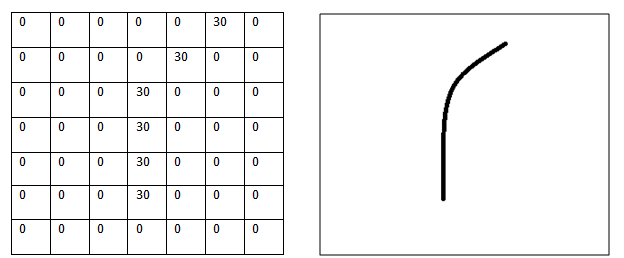
\includegraphics[width=0.95\textwidth]{Filter.png}
       \\
    \only{\tiny{Kernel \\ \url{https://adeshpande3.github.io/} }}
\end{frame}

\begin{frame}
  \frametitle{Convolutional Layers}
  \begin{itemize}
	\item Convolutional Layers are where CNNs get their name
	\pause
	\item Every CNN starts with a convolutional layer
	\pause
	\item The Kernel slides or "convolves" around the input image
	\pause
	\item The results of the convolutions are stored in the feature map
  \end{itemize}
\end{frame}

\begin{frame}
  \frametitle{Convolutional Layers}
   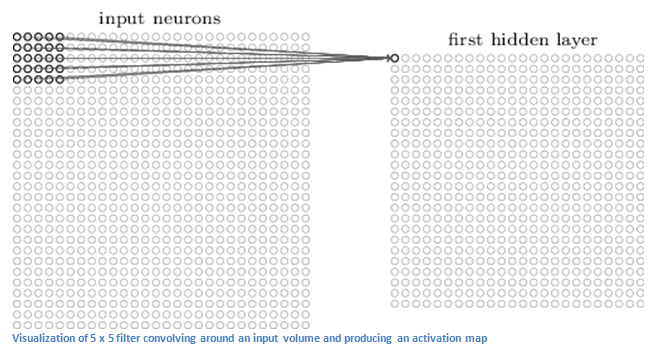
\includegraphics[width=0.95\textwidth]{ActivationMap.png}
       \\
    \only{\tiny{Feature Map \\ \url{https://adeshpande3.github.io/} }}
\end{frame}

\begin{frame}
  \frametitle{Fully Connected Layers} 
  \begin{itemize}
	\item Can be thought of as the final layers in the network
	\pause
	\item Their job is to convert the feature maps from previous layers into label probabilities.
	\pause
	\item these probabilities come in the form of a vector that adds up to 1.
	
  \end{itemize}
\end{frame}

\begin{frame}
  \frametitle{Training}
  \begin{itemize}
	\item Training is the crux that makes everything work
	\pause
	\item Training requires data that has already been properly segmented.
	\pause
	\item Network is initialized with random kernel weights
	\pause
	\item Training has four main steps:
	\pause
	\begin{itemize}
	  \item The forward pass
	  \pause
	  \item The loss calculation
	  \pause
	  \item The backward pass
	  \pause
	  \item Weight update
	\end{itemize}
  \end{itemize}
\end{frame}

\section*{Methods}

\subsection*{Havaei, et al.}

\begin{frame}
  \frametitle{Overview of Havaei, et al.}
  \begin{itemize}
	\item Havaei, et al proposes a two pathway approach to the BRATS 2013 brain tumor segmentation challenge.
	\pause
	\item Their approach has three main components
	\pause
	\begin{itemize}
	  \item Two pathways
	  \pause
	  \item Two CNNs concatenated together
	  \pause
	  \item A two phase approach to training
	\end{itemize}
  \end{itemize}
\end{frame}

\begin{frame}
  \frametitle{Two Pathways}
  \begin{itemize}
	\item Havaei, et al. setup their network with two pathways
	\pause
	\begin{itemize}
	  \item The local pathway with a smaller 7x7 receptive field'
	  \item The global pathway with a larger 13x13 receptive field.
	\end{itemize}
	\pause
	\item These two pathways allow the combination of finite detail with greater locational context.
  \end{itemize}
\end{frame}

\begin{frame}
  \frametitle{Two Pathways}
  \includegraphics[width=1\textwidth]{"../Sample_paper/Two-Pathway".pdf}
\end{frame}

\begin{frame}
  \frametitle{Cascaded Architectures}
  \begin{itemize}
	\item The second approach implemented by Havaei, et al. is their use of a 'cascaded architecture'.
	\pause
	\item In this approach they take the output one of one CNN and concatenate it into a layer of another.
	\pause
	\item The goal is to allow for joint segmentation models where different labels are allowed to correlate with one another.
  \end{itemize}
\end{frame}

\begin{frame}
  \frametitle{Cascaded Architectures}
  \includegraphics[width=0.5\textwidth]{"../Sample_paper/Cascaded Architectures".pdf}
\end{frame}

\begin{frame}
  \frametitle{Two Phase Training}
  \begin{itemize}
	\item The last approach implemented by Havaei, et al. is a two phase training system.
	\pause
	\item This is done to alleviate the relative abundance of healthy tissue versus the small quantity of tumor tissue in each image.
	\item The two phases consist of:
	\pause
	\begin{itemize}
	  \item First they train the network on image patches where the probability of each label being present is equal.
	  \item Then they retrain the final layer with the relative probabilities of each label.
	\end{itemize}
	\pause
	\item This allows for better label discrimination while maintaining proper output probabilities.
  \end{itemize}
\end{frame}

\subsection*{Kamnitsas, et al.}

\begin{frame}
  \frametitle{Overview of Kamnitsas, et al.}
  \begin{itemize}
	\item Kamnitsas, et al have five different architecture approaches
	\pause
	\begin{itemize}
	  \item 3D kernels
	  \pause
	  \item Dense training
	  \pause
	  \item Two pathways
	  \pause
	  \item Deeper networks
	  \pause
	  \item 3D conditional random fields on the output
	\end{itemize}
  \end{itemize}
\end{frame}

\end{document}


